\documentclass{article}
\usepackage{amsmath, amssymb}
\usepackage{pgfplots}
\usepackage{mathhint}

\begin{document}

% Set the context for this problem - this information appears in the page header
% and helps the hint system understand what material you've covered
\mathhintcontext{
  book=Guckenheimer and Holmes,
  chapter=1,
  section=1.0-1.1,
  problem=4,
  lectures={lecture_1.tex, lecture_2.tex}
}

\begin{problem}
\noindent
(30 points) The following equations describe the motion of a ball in a spinning circular hoop, where $\alpha$ is the (nondimensional) speed of the spinning hoop, $\beta$ is the (nondimensional) damping, $x$ is the angle of the ball in the hoop, and $y$ is the ball's angular velocity:
\begin{align*}
  \dot{x}&=y\\
  \dot{y}&=(\alpha \cos x-1)\sin x -\beta y,
\end{align*}
\begin{enumerate}
  \item[(a)] Find the equilibrium points, as a function of the parameters $\alpha$, $\beta$ (consider $x\in[-\pi, \pi]$). Make a sketch of these equilibrium points as a function of $\alpha$. (Such a plot is the beginning of a bifurcation diagram).
  \item[(b)] Show that, for $\beta=0$, the system is Hamiltonian: that is, there is a function $H(x,y)$ such that\begin{align*}
    \dot{x}&=\frac{\partial H}{\partial y}\\
    \dot{y}&=-\frac{\partial H}{\partial x}.
  \end{align*}
  \item[(c)] Fix $\alpha=2$, and consider the stability of each of the equilibrium points you found in part (a). Be sure to consider the cases $\beta<0$, $\beta=0$, and $\beta>0$. [\textit{Hint:} How does the Hamiltonian $H$ vary along trajectories $(x(t),y(t))$ that satisfy the dynamics?]
\end{enumerate}

\end{problem}

\begin{notes}
\paragraph{Part (a)}
Let's start by setting everything equal to 0
\begin{align*}
  0&=y\\
  0&=(\alpha \cos x-1)\sin x -\beta y.
\end{align*}
Hence, 
\[0=(\alpha \cos x-1)\sin x\]
We know that $\sin x=0$ when $x=-\pi,0,+\pi$. For the $\alpha \cos x-1$ we can write 
\begin{gather*}
  \alpha \cos x_0-1=0\\
  \cos x_0 = \frac{1}{\alpha}\\
  x_0 =\pm \arccos\frac{1}{\alpha}
\end{gather*}
where $\arccos$ is only defined for inputs in the range of $[-1,1]$. Hence, $x_0$ will only exist when $\alpha\leq -1$ or $\alpha\geq 1$.

Hence, we have at most five equilibrium points at 
\[x_0=-\pi,-\arccos\frac{1}{\alpha},0,+\arccos\frac{1}{\alpha},+\pi\]
with the equilibrium points that depend on $\alpha$ disappearing if $-1<\alpha<1$. Here is a sketch of these equilibrium points as a function of $\alpha$:

\begin{figure}[h]
\centering
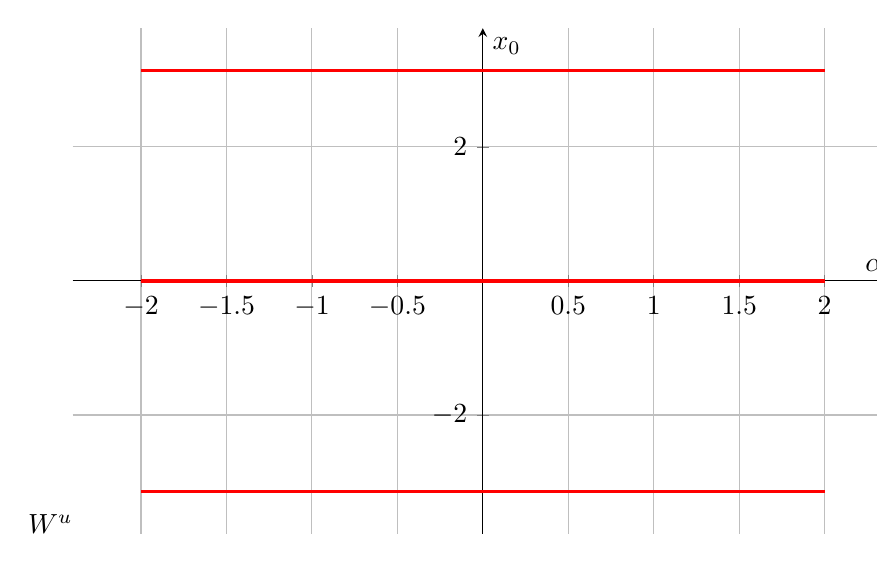
\begin{tikzpicture}
\begin{axis}[
  xlabel={$\alpha$},
  ylabel={$x_0$},
  grid=major,
  width=12cm,
  height=8cm,
  domain=-2:2,
  samples=200,
  axis lines=middle,
  enlargelimits=true,
]
%\addplot[red, very thick] {arccos(1/x)};
%\addplot[red, very thick] {-arccos(1/x)};
\addplot[red, very thick] {0};$W^{u}$
\addplot[red, very thick] {-pi};
\addplot[red, very thick] {pi};
\end{axis}
\end{tikzpicture}
\caption{Plot of equilibrium points as a function of $\alpha$}
\end{figure}

Hmm, I can't get the $\arccos$ functions to render because of the domain issue. Any insight?


\mathhint{Nudge}{2026-02-03 17:40}{Your analysis of the equilibrium points is correct! You've identified all the equilibrium points and their dependence on $\alpha$. 

For the plotting issue: instead of trying to plot the $\arccos$ function directly (which has domain issues), consider plotting the curves in the regions where they're defined - you might want to restrict the domain or use different plot commands for $|\alpha| \geq 1$ versus $|\alpha| < 1$.}

\begin{figure}[h]
\centering
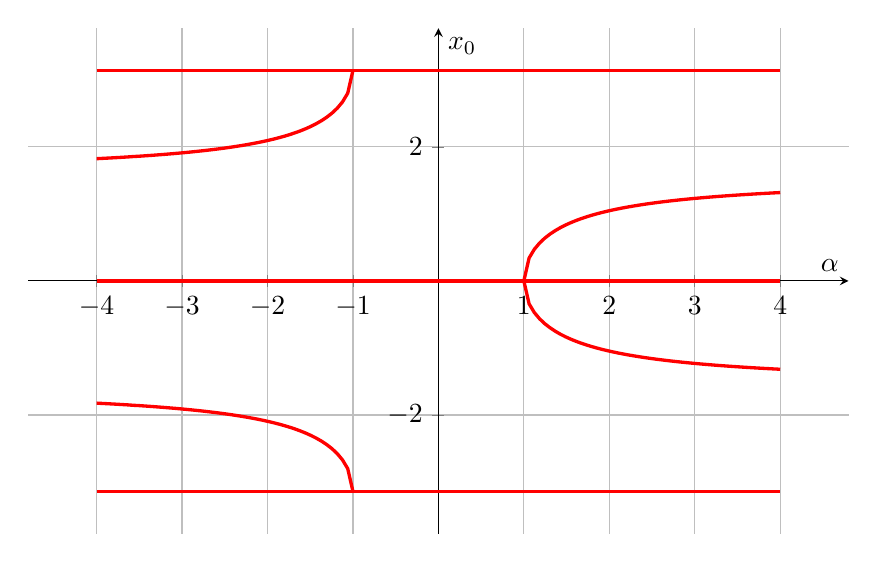
\begin{tikzpicture}
\begin{axis}[
  xlabel={$\alpha$},
  ylabel={$x_0$},
  grid=major,
  width=12cm,
  height=8cm,
  domain=-4:4,
  samples=200,
  axis lines=middle,
  enlargelimits=true,
]
\addplot[red, very thick, domain=1:4, samples=50] {pi*acos(1/x)/180};
\addplot[red, very thick, domain=1:4, samples=50] {-pi*acos(1/x)/180};
\addplot[red, very thick, domain=-4:-1, samples=50] {pi*acos(1/x)/180};
\addplot[red, very thick, domain=-4:-1, samples=50] {-pi*acos(1/x)/180};

\addplot[red, very thick] {0};
\addplot[red, very thick] {-pi};
\addplot[red, very thick] {pi};
\end{axis}
\end{tikzpicture}
\caption{Plot of equilibrium points as a function of $\alpha$}
\end{figure}

Okay this should look correct.

\paragraph{Part (b)}
Let's start by writing 
\begin{align*}
  \frac{\partial H}{\partial y} &= y\\
  \int \partial H &= \int y \partial y 
\end{align*}
where integrating both sides with respect to $y$ yields
\[ H(x,y)= \frac{y^2}{2} + f(x). \]
To identify $f(x)$, we can write 
\begin{align*}
  \frac{\partial H}{\partial x} &= (\alpha \cos x-1)\sin x\\
  \int \partial H &= -\int(\alpha \cos x-1)\sin x \partial x\\
  H(x,y) &= -\int \alpha\cos(x)\sin(x)-\sin x \partial x\\
  H(x,y) &= -\int \frac{\alpha}{2}\sin(2x)-\sin x \partial x\\
  H(x,y) &= -\frac{\alpha}{4}\cos(2x)+\cos(x) + f(y)
\end{align*}
Where our Hamiltonian is
\[ H(x,y)= -\frac{\alpha}{4}\cos(2x)+\cos(x)+\frac{y^2}{2}.\]

\mathhint{Nudge}{2026-02-03 17:55}{Good work on the plotting fix - your bifurcation diagram now correctly shows how the equilibrium points appear and disappear as $\alpha$ varies!

For part (b), your approach to finding the Hamiltonian is on the right track, but double-check your calculation of the integral $\int (\alpha \cos x - 1)\sin x \, dx$ - you might want to verify this step carefully.}

\begin{align*}
  -\frac{\partial H}{\partial x} &= (\alpha \cos x-1)\sin x\\
  \int \partial H &= -\int(\alpha \cos x-1)\sin x \partial x\\
  H(x,y) &= -\int \alpha\cos(x)\sin(x)-\sin x \partial x\\
  H(x,y) &= \int -\alpha\cos(x)\sin(x)\partial x+ \int \sin x \partial x\\
\end{align*}

Should I just use u-substition instead of a trig identity?

\mathhint{Nudge}{2026-02-03 18:00}{Your approach to constructing the Hamiltonian is correct, and you've set up the partial derivative conditions properly. However, there's a sign error in your integration - when you have $\dot{y} = -\frac{\partial H}{\partial x}$, be careful about the negative sign when integrating.}

\begin{align*}
  -\frac{\partial H}{\partial x} &= (\alpha \cos x-1)\sin x\\
  \int \partial H &= -\int(\alpha \cos x-1)\sin x \partial x\\
  H(x,y) &= -\int \alpha\cos(x)\sin(x)-\sin x \partial x\\
  H(x,y) &= \int -\alpha\cos(x)\sin(x)\partial x+ \int \sin x \partial x\\
  H(x,y) &=\int-\alpha u\partial u -\cos x + f(y)\\
  H(x,y) &= -\frac{\alpha \sin^2x}{2}-\cos x + f(y)
\end{align*}
and now our Hamiltonian is 
\[ H(x,y)= \frac{y^2}{2}-\frac{\alpha \sin^2x}{2}-\cos x \]

\mathhint{Nudge}{2026-02-04 13:39}{You're making good progress with the integration! Your use of substitution with $u = \sin x$ is a smart approach, and you're correctly handling the negative signs now. Your final Hamiltonian looks right - you might want to double-check that it satisfies both partial derivative conditions to confirm your work.}

Just as a sanity check, let's compute the partial derivatives to show that this is the correct Hamiltonian. For $\dot{x}$, we can write 
\begin{align*}
  \frac{\partial H}{\partial y}&=y=\dot{x}
\end{align*}
For $\dot{y}$, we can write 
\begin{align*}
  \frac{\partial H}{\partial x}&=-\alpha\sin x \cos x + \sin x\\
  &= -(\alpha\cos x -1)\sin x=-\dot{y}
\end{align*}

\paragraph{Part (c)}
We are given the following hint: ``How does the Hamiltonian $H$ vary along trajectories $(x(t),y(t))$ that satisfy the dynamics?'' But this hint is weird because our Hamiltonian was under the assumption that $\beta=0$ and now we have to incorporate $\beta$ back in.

\mathhint{Nudge}{2026-02-04 13:54}{For part (c), the hint is actually quite insightful even though $\beta \neq 0$ now - think about what happens to $H(x(t), y(t))$ when you differentiate it with respect to time along a solution trajectory of the original system (with $\beta$ included).}

Differentiating our Hamiltonian with respect to time (with $\alpha=2$), we have
\begin{align*}
  \frac{d}{dt}H(x,y)&=y\dot{y}+\left( -2\sin x\cos x +\sin x \right)\dot{x}\\
  &=\left((2 \cos x-1)\sin x -\beta y\right)y - \left(2 \cos x-1\right)\sin x \cdot y\\
  &=(2 \cos x-1)\sin x\cdot y -\beta y^2 - \left(2 \cos x-1\right)\sin x \cdot y\\
  &=-\beta y^2
\end{align*}
Okay this seems nice, if not a little obvious given how we constructed the Hamiltonian. This says that the Hamiltonian depends on $\beta$ and $y$. If $beta>0$, then the Hamiltonian decreases when $y\neq 0$. If $\beta=0$, then the Hamiltonian never decreases and we travel along level sets. If $\beta<0$, then the Hamiltonian always increases when $y\neq 0$. 

But, what does this say about the equilibria?

\mathhint{Nudge}{2026-02-04 15:14}{You've correctly computed how the Hamiltonian changes along trajectories - that's a key insight! Now think about what this behavior of $H(x(t), y(t))$ tells you about the long-term fate of trajectories near equilibrium points, especially considering that equilibria are where $y = 0$.}

I guess we could just make our Hamiltonian equation into a Lyapunov function. First let's evaluate the Hamiltonian at our equilibria
\[x_0=-\pi,-\arccos\frac{1}{\alpha}=-\frac{\pi}{3},0,\arccos\frac{1}{\alpha}=\frac{\pi}{3},\pi\]
We have 
\begin{align*}
  H\left(-\pi,0\right)&=\frac{0^2}{2}-\sin^2(-\pi)-\cos(-\pi)=1\\
  H\left(-\frac{\pi}{3},0\right)&=\frac{0^2}{2}-\sin^2(-\pi/3)-\cos(-\pi/3)=-\left(-\frac{\sqrt{3}}{2}\right)^2-\frac{1}{2}=-\frac{5}{4}\\
  H\left(0,0\right)&=\frac{0^2}{2}-\sin^20-\cos0=-1\\
  H\left(\frac{\pi}{3},0\right)&=\frac{0^2}{2}-\sin^2(\pi/3)-\cos(\pi/3)=-\left(\frac{\sqrt{3}}{2}\right)^2-\frac{1}{2}=-\frac{5}{4}\\
  H\left(\pi,0\right)&=\frac{0^2}{2}-\sin^2(\pi)-\cos(\pi)=1
\end{align*}
So $(-\frac{\pi}{3},0),(\frac{\pi}{3},0)$ have the lowest ``energy''. Could we just make some function 
\[ V(x,y)=\frac{y^2}{2}-\sin^2x-\cos x+\frac{5}{4} \]
and then use a Lyapunov argument that $(-\frac{\pi}{3},0),(\frac{\pi}{3},0)$ are stable equilibria since the $V=0$ and $\dot{V}=0$ at those points? We could also use LaSalle's invariance principle to argue that they are asymptotically stable.

\mathhint{Nudge}{2026-02-04 16:08}{You're getting very close! Your calculation of the Hamiltonian values at equilibria is correct, and you're thinking in the right direction about using the Hamiltonian to analyze stability.

However, consider what happens when $\beta < 0$ - if $\frac{dH}{dt} = -\beta y^2 > 0$ when $y \neq 0$, this means trajectories are moving to *higher* energy levels, which might destabilize certain equilibria.}

Would it be that 
\begin{itemize}
  \item for $\beta > 0$, then the Hamiltonian decreases and we get asymptotic stability for points $(-\frac{\pi}{3},0)$, $(\frac{\pi}{3},0)$ and instability for $(-\pi,0)$,$(0,0)$, and $(\pi,0)$,
  \item for $\beta = 0$, then the Hamiltonian never changes and we get Lyapunov stability for points $(-\frac{\pi}{3},0),(\frac{\pi}{3},0),(-\pi,0),(0,0),(\pi,0)$,
  \item for $\beta < 0$, then the Hamiltonian decreases and we get asymptotic stability for points $(-\pi,0)$, $(0,0)$, and $(\pi,0)$ and instability for $(-\frac{\pi}{3},0)$ and $(\frac{\pi}{3},0)$?
\end{itemize}


\mathhint{Nudge}{2026-02-04 16:24}{You're very close to the complete picture! Your understanding of how the different values of $\beta$ affect stability is correct - when $\beta > 0$, trajectories move to lower energy levels (favoring the low-energy equilibria), and when $\beta < 0$, trajectories move to higher energy levels (favoring the high-energy equilibria).

However, be a bit more careful about the $\beta = 0$ case - just because the Hamiltonian is conserved doesn't automatically guarantee Lyapunov stability for all equilibria.}

Ah okay, I can see how I can make my arguments more precise. Let's try this:

\subparagraph{$\beta>0$}
For our Lyapunov function 
\[ V(x,y)=\frac{y^2}{2}-\sin^2x-\cos x+\frac{5}{4} \]
we have $V=0$ for $(-\frac{\pi}{3},0)$, $(\frac{\pi}{3},0)$ and $\dot{V}\leq 0$, hence these points are suggested to be Lyapunov stable. To show that these are asymptotically, consider the set 
\[ S=\left\{(x,0): x\in\left[-\pi,\pi\right]\right\} \]
where $\dot{V}(S)=0$. However, for points $s\in S$ where $s\notin \left\{(-\frac{\pi}{3},0),(\frac{\pi}{3},0),(-\pi,0),(0,0),(\pi,0)\right\}$ the expression 
\[ \dot{y}=(s\cos x-1)\sin x \]
is not $0$, meaning that trajectories with $(x(t'),y(t'))=s$ for some $t'$ will immediately leave the set $S$. Hence, $S$ is only invariant for trajectories starting at $(-\frac{\pi}{3},0),(\frac{\pi}{3},0),(-\pi,0),(0,0),(\pi,0)$. Via La Salle's invariance principle, it follows that $(-\frac{\pi}{3},0)$, $(\frac{\pi}{3},0)$ are asymptotically stable.

To show that the points $(-\pi,0)$,$(0,0)$, and $(\pi,0)$ are unstable, let's perform a linearization. To start, let's compute $Df(x)$ by writing 
\[ J_f(x,y) = \begin{bmatrix}
\frac{\partial f_1}{\partial x} & \frac{\partial f_1}{\partial y} \\
\frac{\partial f_2}{\partial x} & \frac{\partial f_2}{\partial y} 
\end{bmatrix} \]
Evaluating each expression, we have 
\begin{gather*}
  \frac{\partial f_1}{\partial x}=0\\
  \frac{\partial f_1}{\partial y}=-1\\
  \frac{\partial f_2}{\partial x}=(-2\sin x)\sin x + (2\cos x -1)\cos x=-2\sin^2x+2\cos^2x-\cos x\\
  \frac{\partial f_2}{\partial y}=-\beta
\end{gather*}
where we will say $g(x)=-2\sin^2x+2\cos^2x-\cos x$. Hence we have 
\[ A = \begin{bmatrix}
0 & 1 \\
g(x) &  -\beta
\end{bmatrix} \]
and computing 
\[ \det\left(A-\lambda I\right)=0\] 
we have
\[ -\lambda(-\beta-\lambda)-g(x)=0 \]
and can write 
\[ \lambda = \frac{-\beta\pm\sqrt{\beta^2+4g(x)}}{2}. \]

\end{notes}

\begin{solution}
\paragraph{Part (a)}
Let's start by setting everything equal to 0
\begin{align*}
  0&=y\\
  0&=(\alpha \cos x-1)\sin x -\beta y.
\end{align*}
Hence, 
\[0=(\alpha \cos x-1)\sin x\]
We know that $\sin x=0$ when $x=-\pi,0,+\pi$. For the $\alpha \cos x-1$ we can write 
\begin{gather*}
  \alpha \cos x_0-1=0\\
  \cos x_0 = \frac{1}{\alpha}\\
  x_0 =\pm \arccos\frac{1}{\alpha}
\end{gather*}
where $\arccos$ is only defined for inputs in the range of $[-1,1]$. Hence, $x_0$ will only exist when $\alpha\leq -1$ or $\alpha\geq 1$.

Hence, we have at most five equilibrium points at 
\[x_0=-\pi,-\arccos\frac{1}{\alpha},0,+\arccos\frac{1}{\alpha},+\pi\]
with the equilibrium points that depend on $\alpha$ disappearing if $-1<\alpha<1$. Here is a sketch of these equilibrium points as a function of $\alpha$:
\begin{figure}[h]
\centering
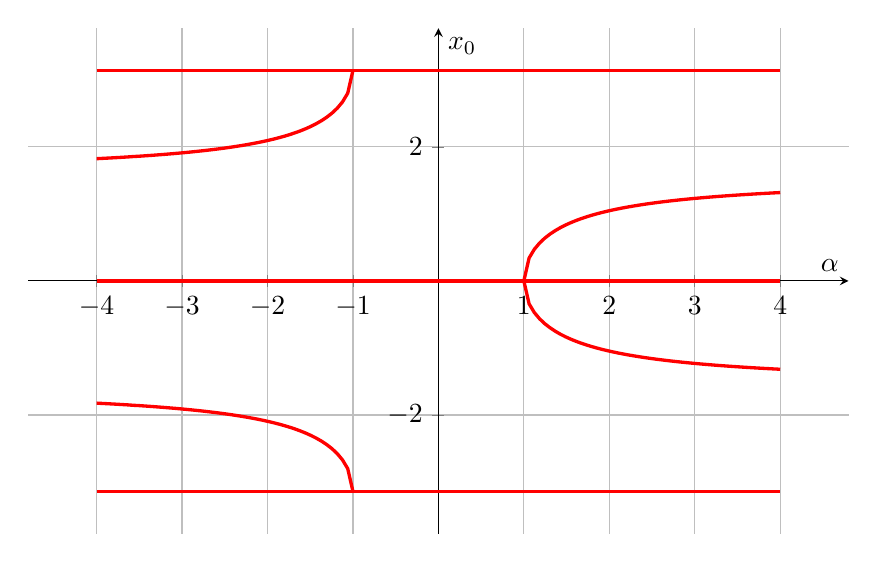
\begin{tikzpicture}
\begin{axis}[
  xlabel={$\alpha$},
  ylabel={$x_0$},
  grid=major,
  width=12cm,
  height=8cm,
  domain=-4:4,
  samples=200,
  axis lines=middle,
  enlargelimits=true,
]
\addplot[red, very thick, domain=1:4, samples=50] {pi*acos(1/x)/180};
\addplot[red, very thick, domain=1:4, samples=50] {-pi*acos(1/x)/180};
\addplot[red, very thick, domain=-4:-1, samples=50] {pi*acos(1/x)/180};
\addplot[red, very thick, domain=-4:-1, samples=50] {-pi*acos(1/x)/180};

\addplot[red, very thick] {0};
\addplot[red, very thick] {-pi};
\addplot[red, very thick] {pi};
\end{axis}
\end{tikzpicture}
\caption{Plot of equilibrium points as a function of $\alpha$}
\end{figure}

\paragraph{Part (b)}
Let's start by writing 
\begin{align*}
  \frac{\partial H}{\partial y} &= y\\
  \int \partial H &= \int y \partial y 
\end{align*}
where integrating both sides with respect to $y$ yields
\[ H(x,y)= \frac{y^2}{2} + f(x). \]
To identify $f(x)$, we can write 
\begin{align*}
  -\frac{\partial H}{\partial x} &= (\alpha \cos x-1)\sin x\\
  \int \partial H &= -\int(\alpha \cos x-1)\sin x \partial x\\
  H(x,y) &= -\int \alpha\cos(x)\sin(x)-\sin x \partial x\\
  H(x,y) &= \int -\alpha\cos(x)\sin(x)\partial x+ \int \sin x \partial x\\
  H(x,y) &=\int-\alpha u\partial u -\cos x + f(y)\\
  H(x,y) &= -\frac{\alpha \sin^2x}{2}-\cos x + f(y)
\end{align*}
and now our Hamiltonian is 
\[ H(x,y)= \frac{y^2}{2}-\frac{\alpha \sin^2x}{2}-\cos x \]

Just as a sanity check, let's compute the partial derivatives to show that this is the correct Hamiltonian. For $\dot{x}$, we can write 
\begin{align*}
  \frac{\partial H}{\partial y}&=y=\dot{x}
\end{align*}
For $\dot{y}$, we can write 
\begin{align*}
  \frac{\partial H}{\partial x}&=-\alpha\sin x \cos x + \sin x\\
  &= -(\alpha\cos x -1)\sin x=-\dot{y}
\end{align*}

\paragraph{Part (c)}
To begin, let's start by performing a linearization. Let's compute $Df(x)$ by writing 
\[ J_f(x,y) = \begin{bmatrix}
\frac{\partial f_1}{\partial x} & \frac{\partial f_1}{\partial y} \\
\frac{\partial f_2}{\partial x} & \frac{\partial f_2}{\partial y} 
\end{bmatrix} \]
Evaluating each expression, we have 
\begin{gather*}
  \frac{\partial f_1}{\partial x}=0\\
  \frac{\partial f_1}{\partial y}=1\\
  \frac{\partial f_2}{\partial x}=(-2\sin x)\sin x + (2\cos x -1)\cos x=-2\sin^2x+2\cos^2x-\cos x\\
  \frac{\partial f_2}{\partial y}=-\beta
\end{gather*}
where we will say $g(x)=-2\sin^2x+2\cos^2x-\cos x$. Hence we have 
\[ A = \begin{bmatrix}
0 & 1 \\
g(x) &  -\beta
\end{bmatrix} \]
and computing 
\[ \det\left(A-\lambda I\right)=0\] 
we have
\[ -\lambda(-\beta-\lambda)-g(x)=0 \]
and can write 
\[ \lambda = \frac{-\beta\pm\sqrt{\beta^2+4g(x)}}{2}. \]
Let's now compute $\lambda$ for each of our equilibria as a function of $\beta$. For $a=2$, we have $\arccos(1/2)=\pi/3$ and we can write 
\begin{center}
\begin{tabular}{c c c c c} 
 $(-\pi,0)$ & $(-\pi/3,0)$ & $(0,0)$ & $(\pi/3,0)$ & $(\pi,0)$ \\[0.5ex] 
 \hline\hline
 $\frac{-\beta\pm\sqrt{\beta^2+4\cdot 3}}{2}$ & $\frac{-\beta\pm\sqrt{\beta^2+4\cdot (-1.5)}}{2}$ & $\frac{-\beta\pm\sqrt{\beta^2+4\cdot 1}}{2}$ & $\frac{-\beta\pm\sqrt{\beta^2+4\cdot (-1.5)}}{2}$ & $\frac{-\beta\pm\sqrt{\beta^2+4\cdot 3}}{2}$ \\ 
\end{tabular}
\end{center}

Now for our equilibria $(-\pi,0),(0,0),(\pi,0)$, we have that our square root quantities ($\sqrt{\beta^2+4\cdot 3}$ and $\sqrt{\beta^2+4\cdot 1}$) are always real and are greater than $|\beta|$. This implies that these equilibria will have at least one positive eigenvalue for all values of $\beta$; hence, $(-\pi,0),(0,0),(\pi,0)$ are unstable for all values of $\beta$.

For our equilibria $(-\pi/3,0),(\pi/3,0)$, the reasoning is more delicate. Let's handle it piecewise.

Let's assume that $\beta>0$. Then we have three cases: $|-6|>\beta^2,|-6|<\beta^2,|-6|=\beta^2$. For the $|-6|=\beta^2$ case, we have $\sqrt{\beta^2-6}=0$ and the equilibria have strictly negative eigenvalues, implying they are asymptotically stable. For the $|-6|>\beta^2$ case, we have $\sqrt{\beta^2-6}$ is an imaginary number and the equilibria have eigenvalues with a strictly negative real part, impying they are asymptotically stable. For the $|-6|<\beta^2$ case, it follows that $|\beta|>\sqrt{\beta^2-6}$, which allows us to write 
\[ -\beta+\sqrt{\beta^2-6}<0 \qquad\text{and}\qquad -\beta-\sqrt{\beta^2-6}<0 \]
Thus the equilibria have eigenvalues with a strictly negative real part, impying they are asymptotically stable. Therefore, in three cases for $\beta>0$, it follows that $(-\pi/3,0),(\pi/3,0)$ are asymptotically stable equilibria.

Let's now assume that $\beta<0$. Then we (again) have three cases: $|-6|>\beta^2,|-6|<\beta^2,|-6|=\beta^2$. For the $|-6|=\beta^2$ case, we have $\sqrt{\beta^2-6}=0$ and the equilibria have strictly positive eigenvalues, implying they are unstable. For the $|-6|>\beta^2$ case, we have $\sqrt{\beta^2-6}$ is an imaginary number and the equilibria have eigenvalues with a strictly positive real part, impying they are unstable. For the $|-6|<\beta^2$ case, it follows that $|\beta|>\sqrt{\beta^2-6}$, which allows us to write 
\[ -\beta+\sqrt{\beta^2-6}>0 \qquad\text{and}\qquad -\beta-\sqrt{\beta^2-6}>0 \]
Thus the equilibria have eigenvalues with a strictly positive real part, impying they are unstable. Therefore, in three cases for $\beta<0$, it follows that $(-\pi/3,0),(\pi/3,0)$ are unstable equilibria.

Let's now assume that $\beta=0$. This is the tricky part, because we get the following expression:
\[ \lambda = \frac{\pm\sqrt{-6}}{2} \]
and we can't conclude anything from the linearization because the real part of our eigenvalues are zero. To make conclusions about the stability, we can turn to the Hamiltonian. As a reminder, with $\alpha=2$, the Hamiltonian is 
\[ H(x,y)= \frac{y^2}{2}- \sin^2x-\cos x \]

First let's evaluate the Hamiltonian at our equilibria to get
\begin{align*}
  H\left(-\pi,0\right)&=\frac{0^2}{2}-\sin^2(-\pi)-\cos(-\pi)=1\\
  H\left(-\frac{\pi}{3},0\right)&=\frac{0^2}{2}-\sin^2(-\pi/3)-\cos(-\pi/3)=-\left(-\frac{\sqrt{3}}{2}\right)^2-\frac{1}{2}=-\frac{5}{4}\\
  H\left(0,0\right)&=\frac{0^2}{2}-\sin^20-\cos0=-1\\
  H\left(\frac{\pi}{3},0\right)&=\frac{0^2}{2}-\sin^2(\pi/3)-\cos(\pi/3)=-\left(\frac{\sqrt{3}}{2}\right)^2-\frac{1}{2}=-\frac{5}{4}\\
  H\left(\pi,0\right)&=\frac{0^2}{2}-\sin^2(\pi)-\cos(\pi)=1
\end{align*}
These values imply that the Hamiltonian has a global minimum of $-\frac{5}{4}$, so in order to make a Lyapunov, we can write 
\[ V(x,y)=\frac{y^2}{2}-\sin^2x-\cos x+\frac{5}{4} \]
Here, it is obvious that $V\left(-\frac{\pi}{3},0\right)=0$ and $V\left(\frac{\pi}{3},0\right)=0$, and that $V>0$ elsewhere. Differentiating our function with respect to time (with $\alpha=2$), we have
\begin{align*}
  \frac{d}{dt}V(x,y)&=y\dot{y}+\left( -2\sin x\cos x +\sin x \right)\dot{x}\\
  &=\left((2 \cos x-1)\sin x -\beta y\right)y - \left(2 \cos x-1\right)\sin x \cdot y\\
  &=(2 \cos x-1)\sin x\cdot y -\beta y^2 - \left(2 \cos x-1\right)\sin x \cdot y\\
  &=-\beta y^2
\end{align*}
and since we have $\beta=0$, it follows that $\dot{V}=0$ everywhere.

From this, we can conclude that for $\beta=0$, the equilibria $(-\pi/3,0),(\pi/3,0)$ are Lyapunov stable. In fact, this makes sense because the derivative of the Hamiltonian being equal to zero implies that orbits travel on level sets. Hence, the equilibria $(-\pi/3,0),(\pi/3,0)$ are centers with trajecories starting sufficiently close to them oscillating around them.

To recap, for all values of $\beta$, we have the following stabilities 
\begin{center}
\begin{tabular}{ |c|c|c|c|c|c| } 
 \hline
  & $(-\pi,0)$ & $(-\pi/3,0)$ & $(0,0)$ & $(\pi/3,0)$ & $(\pi,0)$\\
 \hline
 $\beta >0$ & unstable & asymptotically stable & unstable & asymptotically stable & unstable \\ 
 $\beta =0$ & unstable & Lyapunov stable & unstable & Lyapunov stable & unstable \\ 
 $\beta <0$ & unstable & unstable & unstable & unstable & unstable \\ 
 \hline
\end{tabular}
\end{center}


\mathsolutioncheck{Partial}{2026-02-05 20:06}{The solution has the right approach and correct equilibrium points, but contains several errors. In part (a), the condition should be $|\alpha| \geq 1$, not $\alpha \leq -1$ or $\alpha \geq 1$. In part (c), there are sign errors in the Jacobian calculation and the final table incorrectly states $\beta < 0$ case twice instead of $\beta < 0$ and $\beta > 0$.}
\end{solution}

\end{document}
